\chapter{Atividades em Moodle}

\index{atividades}

\section{Introdução}

As Atividades são as ferramentas Moodle que permitem e estimulam a participação e interação entre os estudantes. São, na visão do autor, as principais ferramentas do ambiente.

Neste capítulo são descritas as principais atividades disponíveis no ambiente Moodle versão 1.9.3$^+$. Apresentam-se, ainda, algumas recomendações sobre a forma de uso de cada uma delas.

Para inserir uma atividade em um curso devem ser repetidos os mesmos primeiros passos dados para inserir recursos: clicar no botão Ativar edição e, escolhida a semana ou tópico, escolher na caixa Acrescentar atividade. Não serão apresentadas todas as atividades disponíveis e nem na ordem que aparecem na caixa de escolha.

\section{Tarefas}

\index{tarefa}

Existem quatro tipos de tarefas no ambiente Moodle. Elas serão aqui apresentadas em ordem de complexidade.

\subsection{Texto online}

\index{texto online}

O texto online é uma tarefa realizada pelos participantes usando o editor html do ambiente Moodle. Escolhendo inserir um texto online aparece a tela mostrada parcialmente na Figura 4.1

\begin{figure}
 \begin{center}
 \fbox{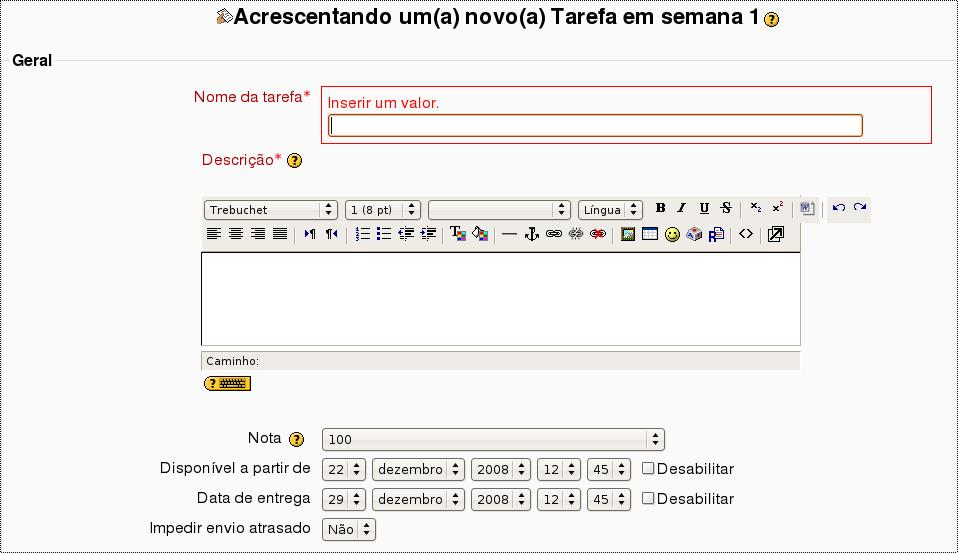
\includegraphics[width=0.95\textwidth]{fig04-01.jpg}}
  \caption{Inserindo um texto online}
 \end{center}
\end{figure}

A Figura 4.2 mostra a parte inferior da tela de configuração de uma tarefa texto online.

\begin{figure}
 \begin{center}
 \fbox{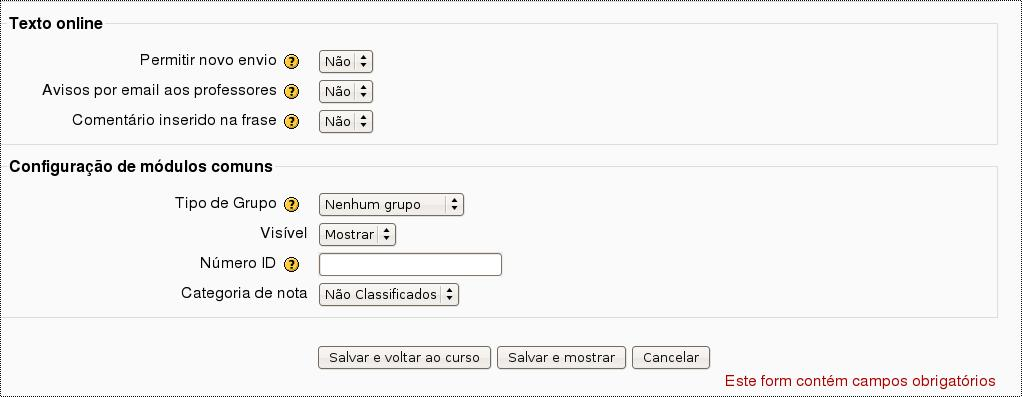
\includegraphics[width=0.95\textwidth]{fig04-02.jpg}}
  \caption{Inserindo um texto online (cont.)}
 \end{center}
\end{figure}

Os campos a serem configurados ou preenchidos são descritos na Tabela 4.1.

\begin{table}
 \begin{center}
  \begin{tabular}{m{4.5cm} m{9.5cm}} \\
  Nome da tarefa & o nome da tarefa como será visto pelos alunos \\
  Descrição & o enunciado da tarefa \\
  Nota & valor máximo da tarefa \\
  Disonível a partir de & data inicial em que a tarefa pode ser realizada \\
  Data de entrega &  Data final para realização da tarefa \\
  Impedir envio atrasado & Permitir ou não a realização da tarefa após da data de entrega \\
  Permitir novo envio & após uma primeira avaliação permitir que o aluno refaça a tarefa \\
  Avisar por email & enviar mensagem por email a cada tarefa enviada \\
  Comentário inserido na frase & feedback do professor no meio do texto do aluno \\
  Tipo de grupo & separação dos alunos em grupos (quando houver) \\
  Visível & tornar ou não a tarefa visível assim que criada \\
  Número ID & identificação da tarefa no quadro de notas \\
  Categoria de nota & classificar a atividade na categoria de nota \\ \hline
 \end{tabular}
 \caption{Criando uma tarefa online}
 \end{center}
\end{table}

Clicando em \textbf{Salvar e voltar ao curso} ou em \textbf{Salvar e mostrar} a tarefa online estará criada.

\subsection{Envio de arquivo único}

\index{Envio de arquivo único}

A tarefa Envio de arquivo único é uma atividade com características muito semelhantes à tarefa online. A diferença é que, em lugar de escrever um texto no editor html do Moodle, o aluno escreve um texto em seu computador e o envia ao ambiente. Há limitações para o tamanho do arquivo e é altamente recomendável que o texto seja enviado no formato rtf \footnote{Rich Text Format ou Formato Rich Text.}. Esse formato pode ser produzido em qualquer editor de textos e tem a grande vantagem de não ser um portador eventual de virus.

Todos os tipos de arquivo podem ser enviados ao ambiente pelos alunos. Fotografias, programas para computador, arquivos comprimidos (zip) ou arquivos proprietários de programas (por exemplo, desenhos em AutoCad).

A configuração de uma tarefa Envio de arquivo único é idêntica àquela do Texto online. A diferença está no lado dos alunos que, em lugar de verem o editor html, verão uma janela para enviar o arquivo produzido em seu computador.

\subsection{Atividade offline}

\index{Atividade offline}

A tarefa do tipo Atividade offline é usada para atribuir notas a trabalhos produzidos pelos alunos em outra forma que não a digital. Seminários, provas presenciais, textos entregues em papel podem ser avaliados e receber um feedback com o uso desta forma de tarefa. Os alunos receberão, por email, um aviso de que a tarefa foi avaliada e poderão ver sua nota e os comentários feitos pelo professor, monitor ou tutor.

\subsection{Modalidade avançada de carregamento de arquivos}

\index{Modalidade avançada de carregamento de arquivos}

Este tipo de tarefa, disponível a partir da versão 1.7 de Moodle, permite que cada aluno envie um ou mais arquivos ao ambiente em qualquer formato.

\subsubsection{Características}

Esta atividade permite que o professor envie arquivos para os alunos em resposta aos trabalhos por eles enviados.

Exemplo: um típico exemplo de uso desta tarefa é o professor editar um trabalho enviado por um aluno, acrescentar comentários e enviar ao aluno para revisão. Quando o aluno clicar no nome da atividade os arquivos enviados para ele aparecem como uma lista de arquivos de resposta.

Os arquivos de resposta podem ser enviados aos alunos antes que eles submetam seus trabalhos. Assim, por exemplo, cada aluno pode ser convidado a trabalhar sobre um texto diferente.

É preciso assegurar que o módulo de Notas (objeto de outro capítulo deste texto) esteja configurado de modo a permitir que as notas e respostas possam ser vistas pelos alunos.

Os aluno podem, também, inserir comentários sobre os textos enviados, sobre o progresso de um trabalho em particular ou qualquer outra informação que desejem.

O envio desta tipo de tarefa deve ser manualmente finalizado pelo aluno.

O professor pode ver a situação de um trabalho a qualquer tempo e os trabalhos não completados são marcados como rascunho.

O professor pode alterar a situação de qualquer trabalho enviado para a situação de rascunho.

\subsubsection{Configuração}

Escolhendo criar uma Modalidade avançada de carregamento de arquivos aparecerá a tela mostrada parcialmente na Figura 4.3.

\begin{figure}
 \begin{center}
 \fbox{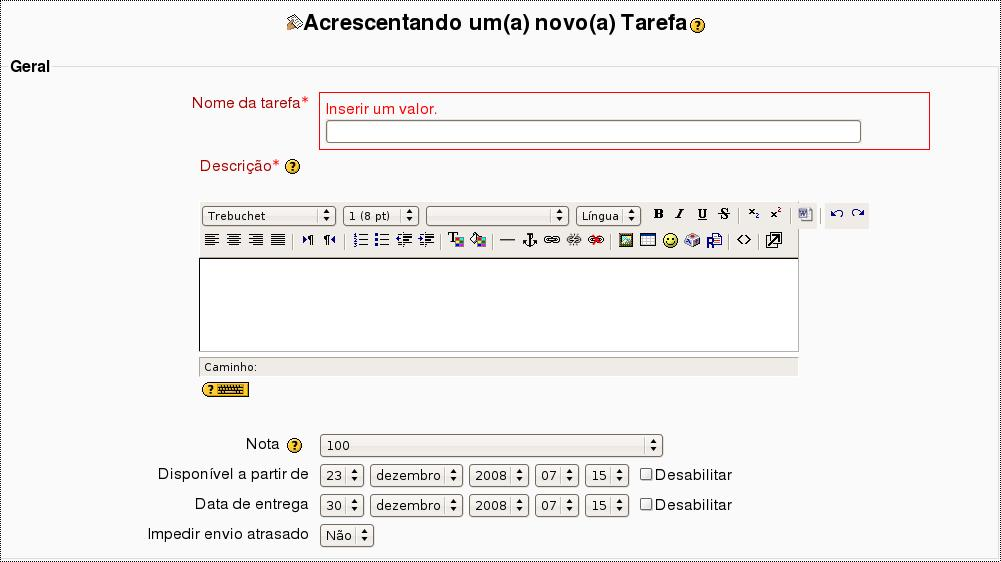
\includegraphics[width=0.95\textwidth]{fig04-03.jpg}}
  \caption{Modalidade avançada de carregamento de arquivos}
 \end{center}
\end{figure}

Os campos mostrados na figura devem ser configurados da mesma forma descrita para os outros tipos de tarefas. As diferenças estão na parte inferior do formulário, mostrada na Figura 4.4.

\begin{figure}
 \begin{center}
 \fbox{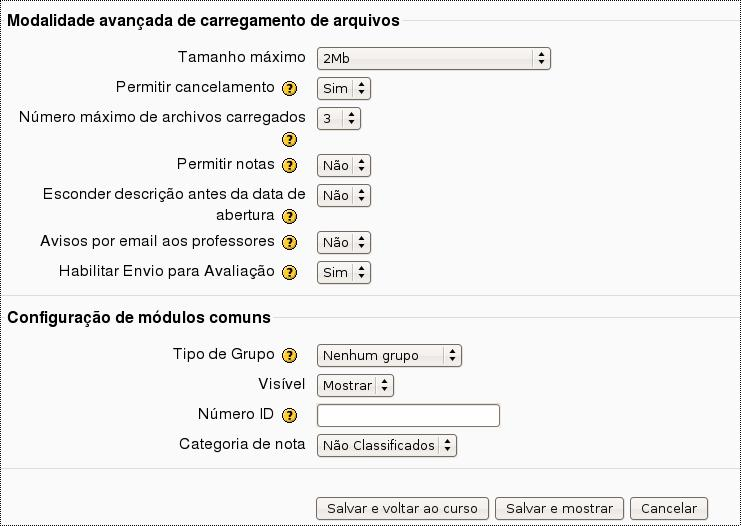
\includegraphics[width=0.95\textwidth]{fig04-04.jpg}}
  \caption{Modalidade avançada de carregamento de arquivos (cont.)}
 \end{center}
\end{figure}

Os campos a serem configurados são descritos na Tabela 4.2

\begin{table}
 \begin{center}
  \begin{tabular}{p{4.5cm} p{9.5cm}} \\
  Tamanho máximo & tamanho máximos dos arquivos que o aluno pode enviar \\
  Permitir cancelamento & Se habilitado, os participantes podem cancelar arquivos enviados a qualquer momento \\
  Número máximo de arquivos & número máximo de arquivos que o aluno pode enviar \\
  Permitir notas & se habilitado, permite que o aluno faça anotações em uma caixa de texto \\
  Esconder descrição &  Se habilitado, a descrição da tarefa não é visualizada antes da data de abertura \\
  Avisos por email & avisar os profesores a cada novo envio de documento ou atualização feita pelos alunos \\
  Permitir novo envio & após uma primeira avaliação permitir que o aluno refaça a tarefa \\
  Avisar por email & enviar mensagem por email a cada tarefa enviada \\
  Habilitar envio para avaliação & O botão "Enviar para avaliação" permite que os usuários comuniquem aos professores que eles terminaram uma tarefa. Os professores podem reverter o status do envio para rascunho (caso o trabalho precise ser melhorado, por exemplo) \\
  Tipo de grupo & separação dos alunos em grupos (quando houver) \\
  Visível & tornar ou não a tarefa visível assim que criada \\
  Número ID & identificação da tarefa no quadro de notas \\
  Categoria de nota & classificar a atividade na categoria de nota \\ \hline
 \end{tabular}
 \caption{Modalidade avançada de carregamento de arquivos}
 \end{center}
\end{table}

\subsection{Avaliando tarefas}

Para ver os trabalhos enviados pelos alunos em uma tarefa clica-se no nome da tarefa para acessar a tela mostrada na Figura 4.5.

\begin{figure}
 \begin{center}
 \fbox{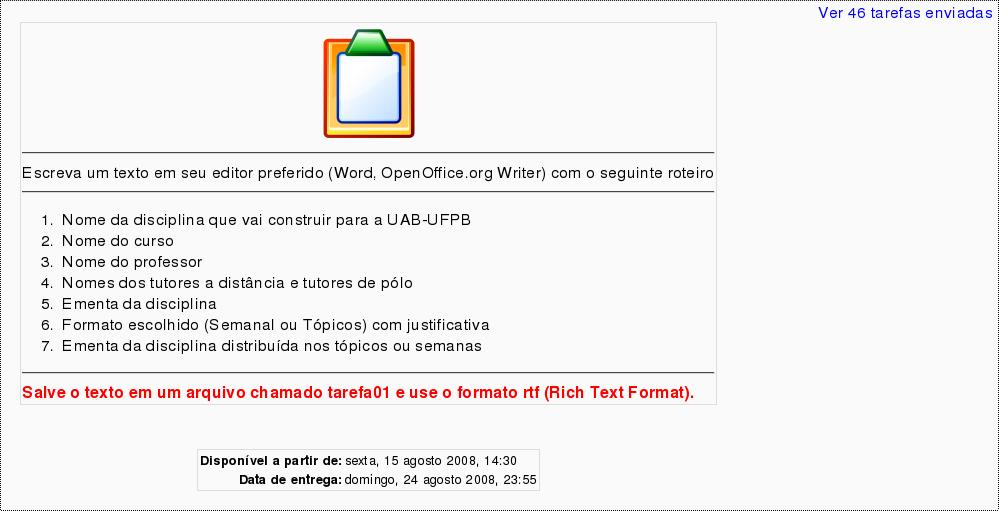
\includegraphics[width=0.95\textwidth]{fig04-05.jpg}}
  \caption{Avaliando tarefas}
 \end{center}
\end{figure}

No alto, à direita, aparece o número de tarefas enviadas. Clique nessa informação e siga os passos a seguir.

\begin{itemize}
 \item Antes de prosseguir é importante observar alguns detalhes. Vá até a parte inferior da tela de avaliações e veja as seguintes informações: Envios por mostrados por página e Permitir avaliação rápida.
\subitem Pode ser interessante colocar um número de avaliações mostradas por página para evitar a necessidade de navegar por muitas telas para ver todos os trabalhos
\subitem Normalmente tem-se que clicar em Nota, à direita do nome de cada aluno, para ver o trabalho enviado, atribuir nota e digitar alguns comentários. Escolhendo Permitir avaliação rápida é possível fazer isso na mesma linha onde está o nome do aluno.
\subitem Feitas as escolhas, clicar em Salvar preferências
\end{itemize}



   3. Before going any further, I would like to draw your attention to some settings on this page. Scroll to the bottom and you will see: Submissions per page and Allow quick grading
         1. I find it useful to set the submissions per page quite large so as not to have to keep opening new pages to see more students.
         2. Normally you have to click on Grade on the right to open a new page where you can view the submission and enter marks and type some feedback text. If you Allow quick grading you can do this on the same line as the submission is listed.
         3. Save preferences if you change either of these. For the rest of this, I will assume that you have enabled Allow quick grading.
   4. On the line across for each person, if they have submited, you will see a link to a file. If you click on the file it will either open in a new browser window (if your browser is capable of viewing the document), or it will ask you if you wish to save to disc or open using the appropriate application program.
   5. Once you have viewed their submission, you can then indicate a mark from the drop down list, and/or enter your comments in the box.
   6. You can do this for many students, however the marks are not stored until you select Save all my feedback either at the top or the bottom of the list of student. It is advisable not to leave too long a time before doing this. After you do this, all students who you left feedback for are sent an email to let them know that there is feedback available for them.
   7. You might note that if you have a long list of students you can sort in many ways, firstname, lastname etc by clicking on the blue link at the top of each column. A useful way is to sort by "Last modified Student" (get the arrow pointing upwards - ie. latest first) which will show the most recently submitted. If you allow more than one submission it is also useful to compare "Last modified student" date with "Last modified Lecturer" date as you can spot who has resubmitted since you last commented.
\section{Laboratório de Avaliação}
O Laboratório de avaliação é uma atividade que permite o envio de documentos pelos estudantes, onde os alunos da disciplina têm acesso a todos os documentos enviados e podem avaliar uns aos outros. O papel do professor nesta atividade é de administrar e atribuir notas à avaliação feita pelos estudantes. Esta atividade suporta uma grande variedade de critérios de avaliação. O professor pode disponibilizar documentos como exemplo para que os alunos pratiquem a avaliação. O Laboratório de avaliação está dividido em cinco fases: configurar fase, fase de envio, fase de avaliação, grading evaluation fase e encerrado.
\subsection{Configurando o laboratório de avaliação}
Para adicionar a atividade laboratório de avaliação, deve-se na disciplina desejada, clicar no botão ativar adição. E então na semana ou tópico desejado, selecionar laboratório de avaliação. Podemos acompanhar esse procedimento a seguir na figura \ref{fig:config_lab}.

\begin{figure}
 \begin{center}
 \fbox{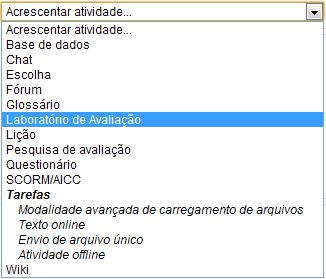
\includegraphics[width=0.4\textwidth]{imagem/cap4/fig_1.jpg}}
  \caption{Acrescentando um laboratório de avaliação}
  \label{fig:config_lab}
 \end{center}
\end{figure}

No passo seguinte encontra-se um formulário, que deve ser preenchido obrigatoriamente nos campos nome do workshop (nome da atividade que ficará visível na plataforma) e introdução (informações gerais sobre a atividade Laboratório de Avaliação).

Na aba recursos do workshop (figura \ref{fig:recursos_work}), pode-se marcar a caixa de seleção em:

\begin{itemize}
 \item “usar exemplos” se desejar submeter um ou mais arquivos como exemplo de como os alunos deverão enviar seus trabalhos.
 \item “use peer assessment” se desejar que os alunos possam avaliar o trabalho dos demais estudantes.
 \item “usar auto-avaliação” se desejar que os alunos possam avaliar seus próprios trabalhos.
\end{itemize}

\begin{figure}
 \begin{center}
 \fbox{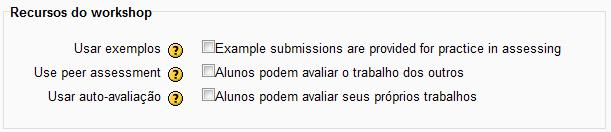
\includegraphics[width=0.6\textwidth]{imagem/cap4/fig_2.jpg}}
  \caption{Recursos do workshop}
  \label{fig:recursos_work}
 \end{center}
\end{figure}

Na aba configurações de nota (figura \ref{fig:config_nota}), pode-se informar em “Nota para envio” a nota máxima que pode ser obtida e a categoria do quadro de notas associada à mesma. Em “Grade de notas” defini-se a nota máxima que pode ser obtida em cada avaliação. No item em “Grading strategy” a estratégia de avaliação a ser utilizada pode ser definida em um dos seguites itens:

\begin{itemize}
 \item Nota acumulativa: comentários e uma nota são dados sobre aspectos específicos;
 \item Comentários - Os comentários são dados sobre aspectos específicos, mas nenhuma nota pode ser atribuída.
 \item Número de erros - Comentários e a seleção de sim/não podem ser avaliados sobre as afirmações especificas;
 \item Rubrica - Um nível de avaliação é dado sobre critérios especificados.
 \end{itemize}

 \begin{figure}
 \begin{center}
 \fbox{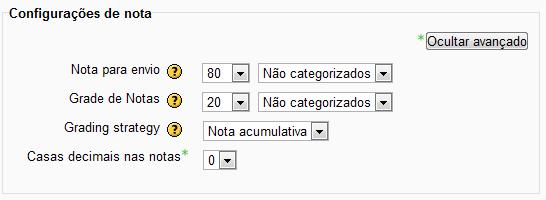
\includegraphics[width=0.6\textwidth]{imagem/cap4/fig_3.jpg}}
  \caption{Configurações de nota}
  \label{fig:config_nota}
 \end{center}
\end{figure}

No item configurações de envio (figura \ref{fig:config_envio}) deve-se preencher o campo “instruções para envio” com informações específicas como quantidade, nome(s), tamanho(s), tipo(s), cores etc. Logo após selecionar o número máximo de anexos enviados, o tamanho máximo de cada arquivo a ser enviado e por fim quando clicar em “Mostrar avançado” pode-se marcar a caixa de seleção “envios atrasados” caso seja necessário permitir o envio de arquivos após o período de tempo estabelecido.

 \begin{figure}
 \begin{center}
 \fbox{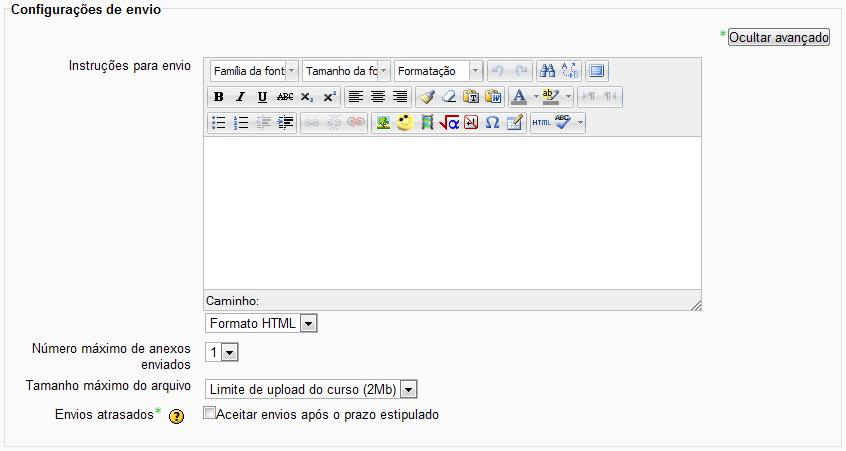
\includegraphics[width=0.6\textwidth]{imagem/cap4/fig_4.jpg}}
  \caption{Configurações de envio}
  \label{fig:config_envio}
 \end{center}
\end{figure}

No item configurações de avaliação (figura \ref{fig:config_ava})temos alguns subitens como “instruções para avaliação” e ao clicar em “Mostrar avançado” podem visualizar “modo de avaliação de exemplos”, caso a opção “usar exemplos” tenha sido marcado anteriormente.

 \begin{figure}
 \begin{center}
 \fbox{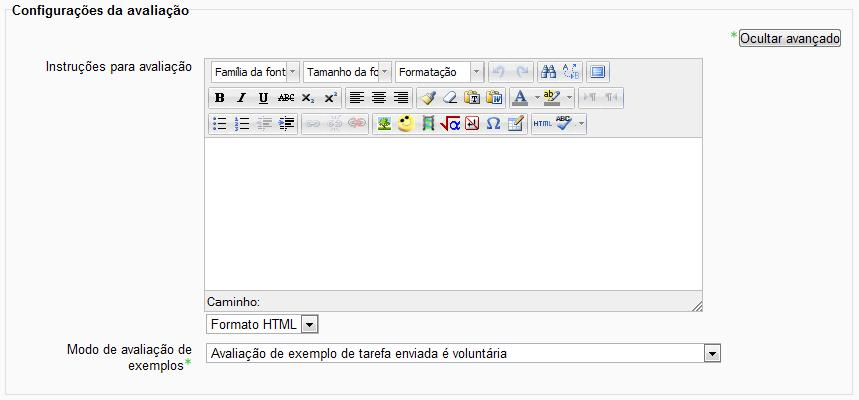
\includegraphics[width=0.6\textwidth]{imagem/cap4/fig_5.jpg}}
  \caption{Configurações de avaliação}
  \label{fig:config_ava}
 \end{center}
\end{figure}

No item “controle de acesso” (figura \ref{fig:controle_acess}) ao clicar em “Mostrar avançado” pode-se visualizar as opções onde será necessário definir a data o horário dos seguintes itens:

\begin{itemize}
 \item Início dos envios: Data e hora do início do envio dos arquivos;
 \item Prazo dos envios: Data e hora final para envio dos arquivos;
 \item Aberto a partir de: Data e hora para início das avaliações;
 \item Prazo da avaliação: Data e hora para o fim das avaliações;
\end{itemize}

\begin{figure}
 \begin{center}
 \fbox{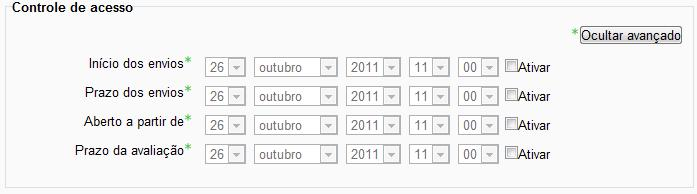
\includegraphics[width=0.6\textwidth]{imagem/cap4/fig_6.jpg}}
  \caption{Controle de acesso}
  \label{fig:controle_acess}
 \end{center}
\end{figure}

No item Configurações comuns de módulos (figura \ref{fig:controle_comum}), no item “Modalidade grupo” deve-se definir uma das seguintes opções:

\begin{itemize}
 \item Nenhum grupo: Não há subgrupos, todos fazem parte de uma grande comunidade.
 \item Grupos separados - Cada membro de grupo pode visualizar apenas seu próprio grupo.
 \item Grupos visíveis - Cada membro do grupo trabalha no seu próprio grupo, mas também pode visualizar outros grupos.
\end{itemize}

\begin{figure}
 \begin{center}
 \fbox{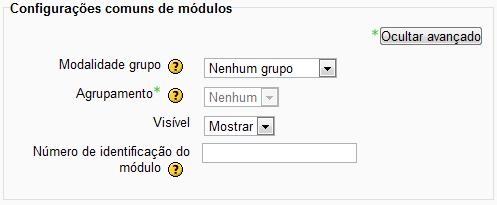
\includegraphics[width=0.6\textwidth]{imagem/cap4/fig_7.jpg}}
  \caption{Configurações comuns de módulos}
  \label{fig:controle_comum}
 \end{center}
\end{figure}

Quando clicar em “Mostrar avançado” pode-se então definir o “Agrupamento”, caso exista, além disto, temos o item “visível” para definir se a atividade ficará visível ou oculta para os estudantes e caso seja necessário, preencher o número de identificação do módulo para fins de avaliação.

Para dar continuidade a criação da atividade Laboratório de Avaliação, deve-se salvar o procedimento e logo após esse comando proceder com a edição do formulário de avaliação. Neste formulário serão definidos pelo professor os aspectos a serem avaliados em relação aos arquivos enviados pelos alunos. O formulário de avaliação varia de acordo com o a opção “Grading strategy”, definida no passo anterior dentro do item configurações de nota. Para cada opção disponível (nota acumulativa, comentários, número de erros e rubrica) um tipo diferente de formulário de avaliação é exibido.

Para preencher o formulário de avaliação, deve-se retornar ao curso onde foram realizados os procedimentos anteriores e clicar sobre a atividade Laboratório de Avaliação criada. Será exibida uma imagem semelhante à figura a seguir:

\begin{figure}
 \begin{center}
 \fbox{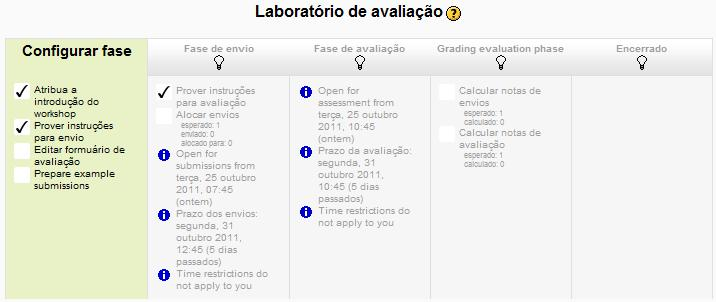
\includegraphics[width=0.6\textwidth]{imagem/cap4/fig_8.jpg}}
  \caption{Edição do laboratório de avaliação}
  \label{fig:edit_lab_ava}
 \end{center}
\end{figure}

Na aba “Configuração fase” deve-se clicar em “editar formulário de avaliação”, em seguida será exibido o formulário de acordo com a opção “Grading strategy” selecionada. Se o item selecionado foi nota acumulativa (figura \ref{fig:item_nota_acumulativa}), será exibido um formulário com os campos semelhantes à figura \ref{fig:edit_lab_ava}.

\begin{figure}
 \begin{center}
 \fbox{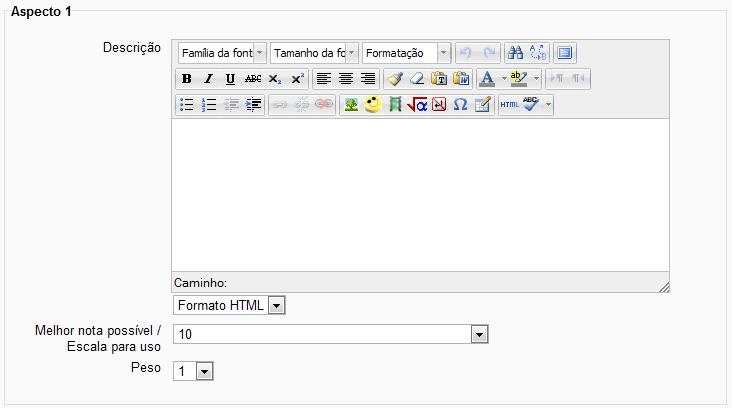
\includegraphics[width=0.6\textwidth]{imagem/cap4/fig_9.jpg}}
  \caption{Item nota acumulativa}
  \label{fig:item_nota_acumulativa}
 \end{center}
\end{figure}

Para cada aspecto a ser avaliado, escrever uma breve descrição, informar a maior nota possível para o aspecto e definir um peso para a nota. Por padrão são exibidos três aspectos, porém, caso seja necessário, é possível adicionar mais aspectos de avaliação clicando-se no botão “Em branco para mais 2 aspectos”. Para finalizar o preenchimento do formulário de avaliação, deve-se clicar no botão salvar.

Se o item escolhido foi comentários será exibido um formulário com os campos semelhantes à figura \ref{fig:item_comentario}. Para cada aspecto a ser avaliado, escrever uma breve descrição. Por padrão são exibidos três aspectos, porém, caso seja necessário, é possível adicionar mais aspectos de avaliação clicando-se no botão “Em branco para mais 2 aspectos”. Para finalizar o preenchimento do formulário de avaliação, deve-se clicar no botão salvar.

\begin{figure}
 \begin{center}
 \fbox{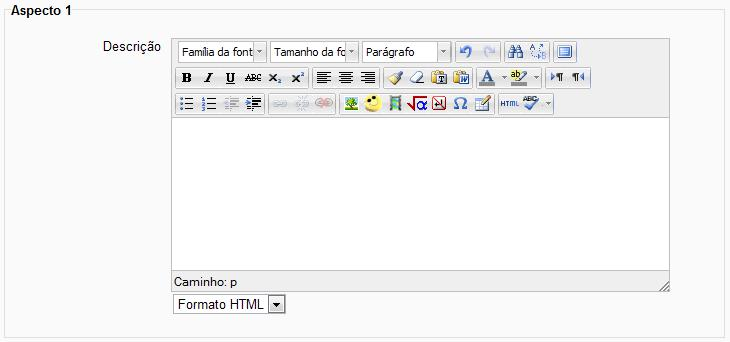
\includegraphics[width=0.6\textwidth]{imagem/cap4/fig_10.jpg}}
  \caption{Item comentário}
  \label{fig:item_comentario}
 \end{center}
\end{figure}


Se o item escolhido foi número de erros será exibido um formulário com os campos semelhantes à figura \ref{fig:item_numero_erro}. Neste tipo de formulário, devem-se elaborar afirmações a cerca dos arquivos enviados pelos estudantes. Para cada afirmação, deve-se estabelecer uma palavra para o erro e outra para o acerto (por exemplo, sim ou não), além de um peso.

\begin{figure}
 \begin{center}
 \fbox{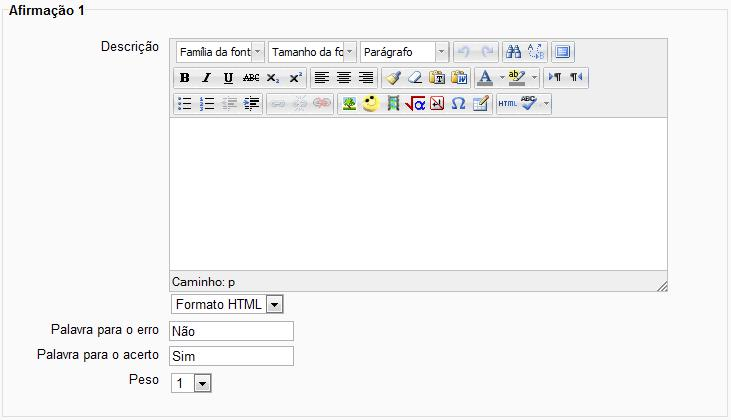
\includegraphics[width=0.6\textwidth]{imagem/cap4/fig_11.jpg}}
  \caption{Item número de erro}
  \label{fig:item_numero_erro}
 \end{center}
\end{figure}

Por padrão são exibidas três afirmações, porém, caso seja necessário, é possível adicionar mais aspectos de avaliação clicando-se no botão “Em branco para mais 2 aspectos”. Para finalizar o preenchimento do formulário de avaliação, deve-se clicar no botão salvar.

\begin{figure}
 \begin{center}
 \fbox{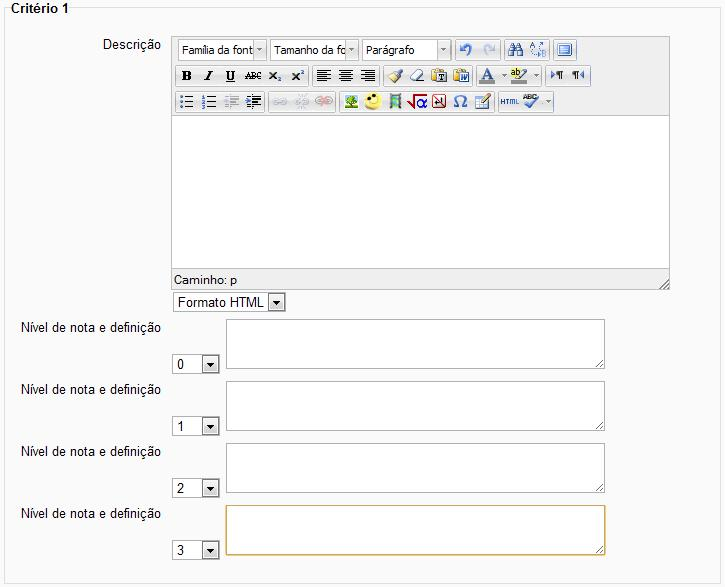
\includegraphics[width=0.6\textwidth]{imagem/cap4/fig_12.jpg}}
  \caption{Critérios de avaliação}
  \label{fig:criterios_ava}
 \end{center}
\end{figure}

Se o item escolhido foi rubrica será exibido um formulário com os campos semelhantes à imagem anterior. Neste tipo de formulário, devem-se elaborar critérios de avaliação (figura \ref{fig:criterios_ava}). Para cada critério, devem-se estabelecer comentários que indiquem níveis de elaboração, além de uma nota associada a cada nível. Não é obrigatório o preenchimento dos quatro níveis apresentados no formulário, em outras palavras, podem-se preencher dois ou três, de acordo com a necessidade da atividade.

Por padrão são exibidos três critérios, porém, caso seja necessário, é possível adicionar mais aspectos de avaliação clicando-se no botão “Em branco para mais 2 aspectos”.

O modo de exibição do formulário de avaliação da rubrica pode ser definido de duas maneiras: grade ou lista. Esta seleção do modo de exibição pode ser realizada no final do preenchimento do formulário, conforme figura \ref{fig:config_rubrica}.

\begin{figure}
 \begin{center}
 \fbox{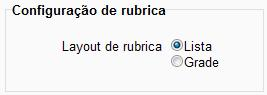
\includegraphics[width=0.6\textwidth]{imagem/cap4/fig_13.jpg}}
  \caption{Configuração de rubrica}
  \label{fig:config_rubrica}
 \end{center}
\end{figure}

Para finalizar o preenchimento do formulário de avaliação, deve-se clicar no botão salvar e sair.

Após a conclusão da escolha e do preenchimento do formulário adequado, é necessária a criação e o envio de arquivos de exemplo para que os estudantes possam tomar como base para a elaboração de seus trabalhos antes de enviar seus arquivos. É importante ressaltar que o envio de exemplos só é possível se a opção “usar exemplos” for selecionada no início da criação desta atividade. Para adicionar arquivos exemplo a esta atividade, após a conclusão do preenchimento do formulário de avaliação, a opção “Exemplo de tarefa enviada” é habilitada. Para adicionar um arquivo de exemplo, basta clicar no botão “Adicionar exemplo de tarefa enviada”, conforme a figura \ref{fig:exe_tarefas}.

\begin{figure}
 \begin{center}
 \fbox{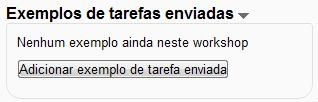
\includegraphics[width=0.6\textwidth]{imagem/cap4/fig_14.jpg}}
  \caption{Exemplos de tarefas enviadas}
  \label{fig:exe_tarefas}
 \end{center}
\end{figure}

Em seguida deve-se preencher o formulário de tarefa enviada, informando um título para o exemplo e clicando-se no botão adicionar para enviar o arquivo de exemplo. É possível adicionar mais de um exemplo de tarefa, porém é importante alertar para o fato de que caso a avaliação dos exemplos esteja habilitada, o estudante poderá avaliar cada exemplo de maneira independente. Para finalizar, deve-se clicar no botão salvar mudanças.

\subsection{Fase de envio}

A fase de envio, como o próprio nome sugere, refere-se à fase onde os alunos estão aptos a enviarem seus arquivos, conforme configurações realizadas na fase anterior. Para habilitar esta fase, independente dos prazos de envio estabelecido, deve-se clicar no ícone fase de envio. Na mensagem seguinte clicar em continuar.

Na alocação de envios (figura \ref{fig:aloc_manual}) o professor deve indicar de forma manual ou aleatória os alunos que poderão se avaliar.

\begin{figure}
 \begin{center}
 \fbox{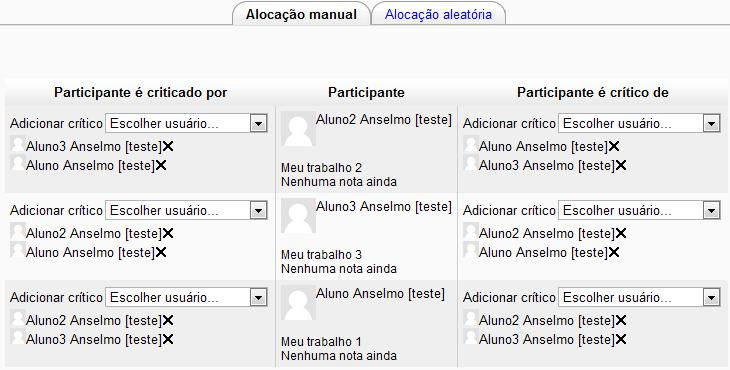
\includegraphics[width=0.6\textwidth]{imagem/cap4/fig_15.jpg}}
  \caption{Alocação manual}
  \label{fig:aloc_manual}
 \end{center}
\end{figure}

Conforme imagem anterior, que ilustra um exemplo de alocação manual, o usuário “Aluno2” pode ter seu trabalho (Meu trabalho 2) criticado pelos usuários “Aluno” e “Aluno3” e criticar os trabalhos enviados pelos usuários “Aluno” e “Aluno 3”.  Da mesma forma, o usuário “Aluno3” pode ter seu trabalho (Meu trabalho 3) criticado pelos usuários “Aluno2” e “Aluno”, como também criticar os trabalhos enviados pelos usuários “Aluno2” e “Aluno”.

De forma semelhante, o usuário “Aluno” pode ter seu trabalho (Meu trabalho 1) criticado pelos usuários “Aluno2” e “Aluno3”, como também criticar os trabalhos enviados pelos usuários “Aluno2” e “Aluno3”. Para modificar manualmente essa configuração, basta excluir o usuário desejado clicando-se no ícone  correspondente ou no botão seletor escolher usuário.

Para alocar a interação de avaliações entre os alunos de forma aleatória, ou seja, de forma automática, deve-se clicar em
Alocação aleatória, conforme a figura (\ref{fig:aloc_aletoria}). Em seguida devem-se configurar as seguintes opções: modalidade de grupo, número de críticos por envio ou número de críticos por participante, se desejar poderá remover as alocações atuais, os participantes podem avaliar os trabalhos enviados pelos demais alunos sem terem enviado o seu próprio trabalho e se for possível o participante avaliar seu próprio trabalho.

\begin{figure}
 \begin{center}
 \fbox{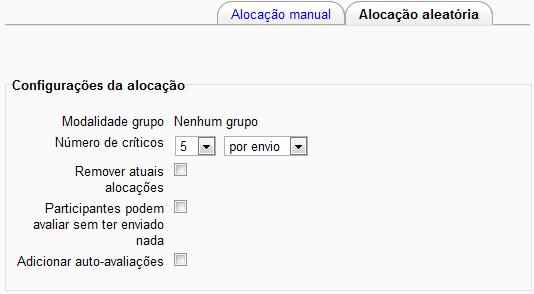
\includegraphics[width=0.6\textwidth]{imagem/cap4/fig_16.jpg}}
  \caption{Alocação aleatoria}
  \label{fig:aloc_aletoria}
 \end{center}
\end{figure}

\subsection{Fase de avaliação}

Para mudar para a fase de avaliação, o professor deve clicar no ícone fase de avaliação. Nesta fase, os alunos poderão avaliar uns aos outros de acordo com as combinações alocadas na fase anterior (Alocação aleatória), podendo também avaliar o exemplo de arquivo enviado pelo professor.

Em \textit{grading evaluation} fase o professor irá verificar as avaliações realizadas pelos alunos, bem como as notas atribuídas aos trabalhos enviados e estabelecer a nota final de cada trabalho.

\begin{figure}
 \begin{center}
 \fbox{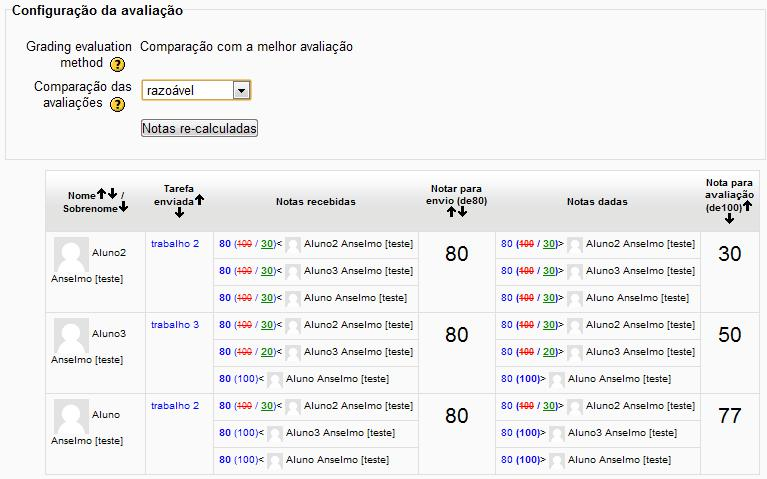
\includegraphics[width=0.6\textwidth]{imagem/cap4/fig_17.jpg}}
  \caption{Configuração da avaliação}
  \label{fig:config_ava2}
 \end{center}
\end{figure}

A figura \ref{fig:config_ava2} indica um exemplo de tarefas enviadas por três alunos. Caso seja interesse do professor, existe a possibilidade de alterar manualmente cada nota atribuída ou recebida por cada aluno, para isso, basta clicar no link onde são exibidas as notas nas colunas Notas recebidas e Notas dadas e sobrepor as notas.

A nota final dos alunos é atribuída de forma automática, no entanto, o professor deve estabelecer o grau de rigidez das avaliações. Para isso, deve-se utilizar a opção Comparação das avaliações para selecionar o grau de rigorosidade muito brando, brando, razoável, rigoroso ou muito rigoroso. Quanto mais rigorosa for à comparação, mais similares às avaliações precisam ser para que se possa obter uma nota alta. Após a seleção do grau de rigorosidade, deve-se clicar em Notas re-calculadas, para que o sistema gere as notas automaticamente.

\subsection{Fase errado}

Indica o encerramento da atividade Laboratório de avaliação. Para mudar para esta fase deve-se clicar em encerrado.

\section{Lição}

A lição é uma atividade que busca direcionar o aluno na medida em que ele responda questões. Uma lição baseia-se em uma página contendo texto, imagem ou vídeo e solicita que o aluno, após a leitura, responda uma determinada questão relacionada ao que foi apresentado. As questões apresentadas podem ser de diversos tipos como múltipla escolha, verdadeiro ou falso, de correspondência, dissertativa, etc. Dependendo da resposta do aluno, ele pode ser conduzido a uma nova página contendo outra questão ou ao final da lição, por exemplo.

Para criar a atividade Lição (figura \ref{fig:add_licao}), temos de ir à disciplina desejada, clicar no botão ativar edição e na semana ou tópico selecionar Lição.

\begin{figure}
 \begin{center}
 \fbox{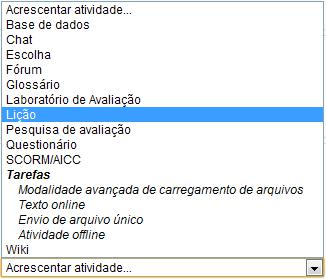
\includegraphics[width=0.6\textwidth]{imagem/cap4/fig_18.jpg}}
  \caption{Adicionar lição}
  \label{fig:add_licao}
 \end{center}
\end{figure}

Após esta escolha será apresentado um formulário, conforme a figura \ref{fig:form_licao}.

\begin{figure}
 \begin{center}
 \fbox{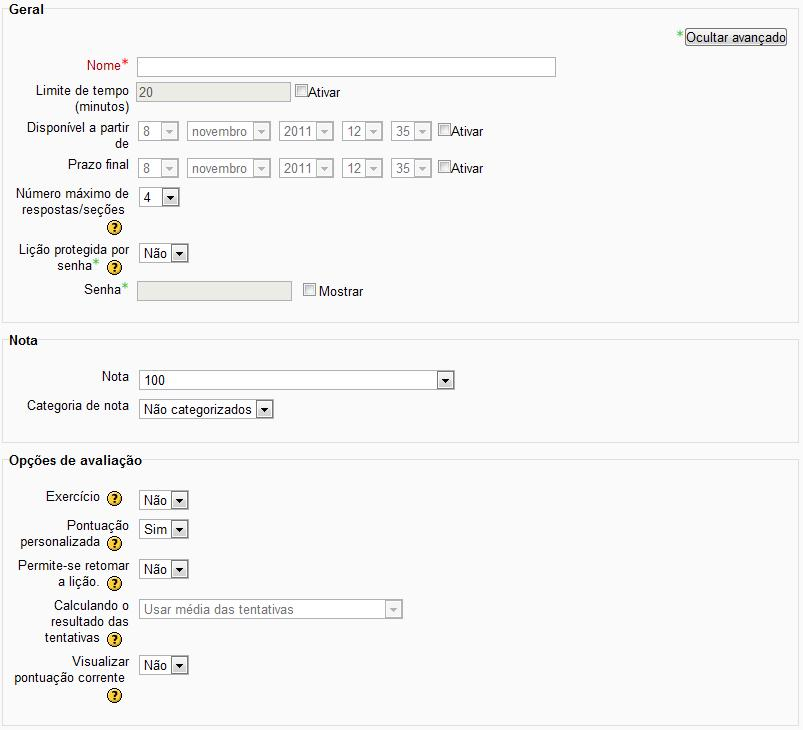
\includegraphics[width=0.7\textwidth]{imagem/cap4/fig_19.jpg}}
  \caption{Formulário de lição}
  \label{fig:form_licao}
 \end{center}
\end{figure}

A seguir podem-se observar os detalhes deste formulário:

\begin{itemize}
 \item \textbf{Nome:} nome da atividade que ficará visível na plataforma;
 \item \textbf{Limite de tempo:} Quantidade de minutos que o aluno terá para responder toda a lição;
 \item \textbf{Disponível a partir de:} data de início do período em que a lição ficará disponível;
 \item \textbf{Prazo final:} data de fim do período em que a lição ficará disponível;
 \item \textbf{Número máximo de respostas/sessões:} número máximo de respostas que o professor pode usar. O valor padrão é 4. Por exemplo, se a lição usar sempre questões VERDADEIRO ou FALSO, é recomendável que este valor seja 2. Esse valor pode ser alterado mesmo após a criação da lição.
 \item \textbf{Nota:} Valor da nota a ser atribuída para a lição;
 \item \textbf{Categoria de nota:} Selecionar a categoria de notas do quadro de notas onde a lição será alocada.
 \item \textbf{Exercício:} Se habilitado, a lição não será avaliada com nota, apenas será criada para fins de estudo;
 \item \textbf{Pontuação personalizada:} Permite que cada resposta da lição tenha uma pontuação diferenciada. Os valores desta pontuação podem ser negativos ou positivos;
 \item \textbf{Permite-se retomar a lição:} Determina se os estudantes poderão realizar a lição mais de uma vez ou somente uma vez. O professor pode decidir que a lição contém material que o estudante deve aprender inteiramente;
 \item \textbf{Calculando o resultado das tentativas:} Caso a opção anterior esteja habilitada, permite escolher se a nota da lição será atribuída como a média das notas das tentativas ou como a nota mais alta;
 \item \textbf{Visualizar pontuação corrente:} Permite ao aluno visualizar os pontos acumulados até este momento, na medida em que for respondendo as perguntas da lição.
\end{itemize}

\begin{figure}
 \begin{center}
 \fbox{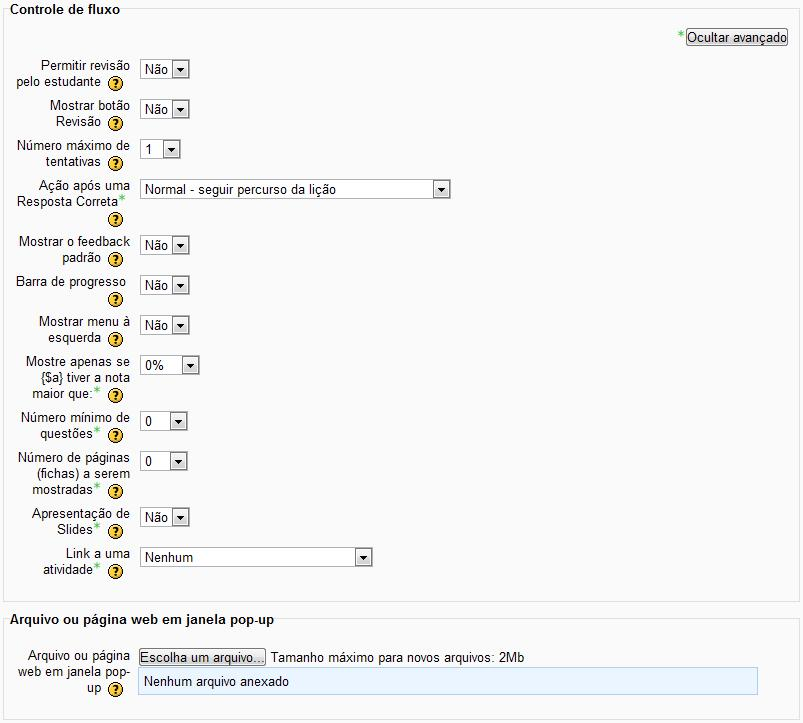
\includegraphics[width=0.6\textwidth]{imagem/cap4/fig_20.jpg}}
  \caption{Controle de fluxo}
  \label{fig:cont_fluxo}
 \end{center}
\end{figure}

A seguir os detalhes referentes a essa tarefa (figura \ref{fig:cont_fluxo}:

\begin{itemize}
 \item \textbf{Permitir revisão pelo estudante:} Se habilitada, permite que o estudante volte atrás na lição, caso necessite modificar suas respostas.
 \item \textbf{Mostrar botão revisão:} Se habilitada, mostra um botão depois de uma questão respondida incorretamente, permitindo que o estudante tente novamente. Esta opção não é compatível com questões dissertativas.
 \item \textbf{Número máximo de tentativas:} Indica o número de tentativas permitidas pelos alunos para realização da lição.
 \item \textbf{Ação após uma Resposta Correta:} A ação mais comum é que a lição siga, na medida em que o aluno responda as questões, de acordo com a ordem especificada em sua criação, porém, é possível modificar esta lógica. A lógica mais comum, citada anteriormente, refere-se à opção Normal. A opção Mostrar uma página nunca vista nunca permite que a mesma página seja mostrada duas vezes (mesmo se o estudante não responder a questão associada corretamente). A outra opção não-padrão é Mostrar uma página não respondida, que permite que os estudantes vejam páginas já navegadas, caso não as questões não tenham sido respondidas corretamente.
 \item \textbf{Mostrar o feedback padrão:} Se selecionado como \textbf{não}, após a conclusão de uma resposta, o usuário será redirecionado para próxima questão, se selecionado como \textbf{sim}, após a conclusão da questão, será exibido um feedback (“Esta é a resposta correta" ou "Esta é a resposta errada") de acordo com a resposta do aluno.
 \item \textbf{Barra de progresso:} Exibe uma barra de progresso na parte inferior da lição.
 \item \textbf{Mostrar menu à esquerda:} Mostra uma lista das páginas (Painel de Navegação) na lição. Mostre apenas se $\{\$a\}$ tiver a nota maior que: Esta configuração determina se um estudante deve obter uma certa nota antes de visualizar o menu à esquerda.
 \item \textbf{Número mínimo de questões:} Quando uma lição contém um ou mais Painéis de Navegação o professor normalmente deve ativar esse parâmetro. O seu valor determina um limite mínimo do número de questões analisadas quando uma média é calculada, mas sem forçar os estudantes a responderem essa quantidade na lição. Por exemplo, alterando esse parâmetro para, digamos, 20, certificaremos que as notas serão dadas como se os alunos tivessem visto \textbf{no mínimo} esse número de questões. Tomemos o caso de um estudante que só viu uma única ramificação na lição, com 5 páginas, e respondeu corretamente todas as questões associadas a ela. Eles podem preferir terminar a lição. Se esse parâmetro estiver desmarcado, a nota dele poderia ser 5 de 5, que é 100\%. Entretanto, definido para 20, sua nota cairia para 5 de 20, que é 25\%.
 \item \textbf{Número de páginas (fichas) a serem mostradas:} O valor padrão é zero, o que significa que todas as Páginas/Fichas são mostradas em uma lição. Fixando o parâmetro com um valor diferente de zero mostra esse número de páginas. Após esse número de Páginas/Fichas terem sido mostradas, o fim da lição é alcançado e a nota é mostrada ao aluno. Se este parâmetro for fixado em um valor maior que o número de páginas na lição, então o final da lição é atingido quando todas as páginas tiverem sido mostradas.
 \item \textbf{Apresentação de slides:} permite a exibição das lições como uma apresentação de slide, com largura e altura fixas e cor do plano de fundo alterável.
 \item \textbf{Link a uma atividade:} A caixa de seleção contém todas as atividades deste curso. Se uma estiver selecionada, então um link para esta atividade aparecerá no final da Lição.
\end{itemize}

\begin{figure}
 \begin{center}
 \fbox{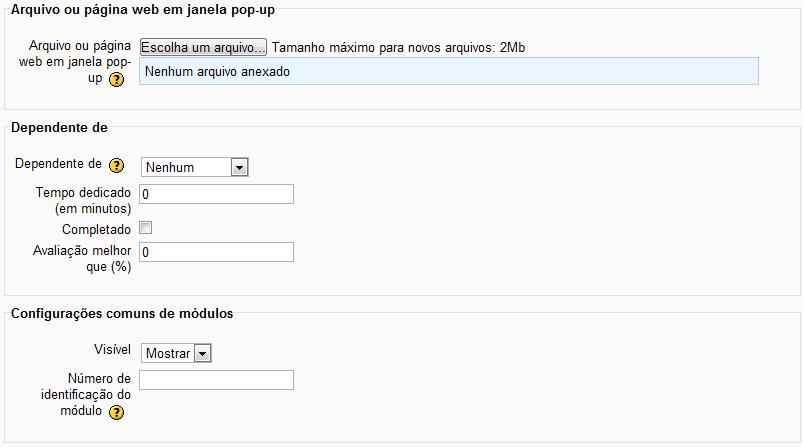
\includegraphics[width=0.6\textwidth]{imagem/cap4/fig_21.jpg}}
  \caption{Configurações de arquivo para uma lição}
  \label{fig:conf_arq_licao}
 \end{center}
\end{figure}


A seguir alguns detalhes sobre as configurações de lição (figura \ref{fig:conf_arq_licao}):

\begin{itemize}
 \item \textbf{Arquivo ou página web em janela pop-up:} No início de uma lição, uma nova janela (pop-up) para uma página web ou um arquivo. Os tipos de arquivo suportados são: mp3, Quicktime, HTML, texto plano, GIF, JPEG e PNG. Outros tipos de formato serão indicados como links para download.
 \item \textbf{Depende de:} Este parâmetro possibilita que esta lição dependa do desempenho do aluno em outra lição do mesmo curso. Se as exigências de desempenho não forem atingidas, o aluno não terá acesso a esta lição. As condições para a dependência incluem:
 \item \textbf{Tempo dedicado:} o aluno deve gastar esta quantidade de tempo estabelecida na lição requerida.
 \item \textbf{Completado:} o aluno deve completar a lição requerida.
 \item \textbf{Avaliação melhor que:} o aluno deve obter uma nota na lição requerida maior que a especificada aqui.
 \item \textbf{Visível:} Se a lição ficará oculta ou não.
 \item \textbf{Número de identificação do módulo:} Número utilizado para fins de avaliação.
\end{itemize}

Após a conclusão e seleção das opções gerais para a criação da atividade Lição, deve-se salvar as configurações realizadas clicando no botão Salvar e voltar para o curso para salvar e retornar para a disciplina ou no botão Salvar e mostrar para salvar e mostrar o recurso criado.

Após a conclusão da etapa anterior, deve-se clicar sobre a lição criada para que as questões possam ser adicionadas. Será exibida a figura \ref{fig:inserindo_quest}.

\begin{figure}
 \begin{center}
 \fbox{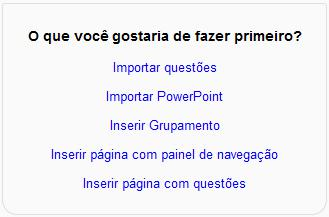
\includegraphics[width=0.6\textwidth]{imagem/cap4/fig_22.jpg}}
  \caption{Inserindo questões na lição}
  \label{fig:inserindo_quest}
 \end{center}
\end{figure}

Como pode ser observado, existem duas opções de importação: questões e PowerPoint. A importação de questões refere-se ao carregamento de questões já criadas previamente. Essas questões devem está presentes no Banco de Questões da disciplina e são as mesmas utilizadas na atividade questionário. A importação do PowerPoint refere-se ao upload de um arquivo com extensão .ppt ou .pptx, ou seja, um arquivo criado pelo software PowerPoint. Ambos os tipos de importação não serão abordados nesta sessão, tendo em vista que dependem de etapas anteriores para serem realizadas.

Grupamento refere-se um tipo de divisão entre as questões de uma lição. Em outras palavras, um grupamento pode ser inserido entre as questões de uma lição para dar um novo destino como, por exemplo, o fim da lição. Para inserir um grupamento deve-se clicar em Inserir Grupamento, a seguir, será apresentada a seguinte imagem.

\begin{figure}
 \begin{center}
 \fbox{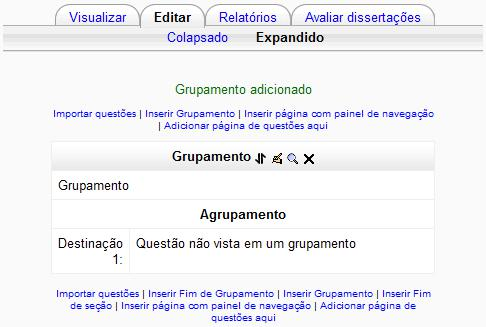
\includegraphics[width=0.6\textwidth]{imagem/cap4/fig_23.jpg}}
  \caption{Inserindo grupamento}
  \label{fig:inserindo_grup}
 \end{center}
\end{figure}

A figura \ref{fig:inserindo_grup} exibe os Agrupamentos de questões existentes na lição. Para inserir um novo grupamento deve-se clicar novamente em Inserir Grupamento. Em seguida, um novo grupamento será criado automaticamente. Para editá-lo basta clicar no ícone
